\subsection{Modelli Compartimentali}

In campo epidemiologico, i modelli compartimentali rappresentano una 
metodologia di modellazione generica che si presta bene all'analisi 
globale del comportamento di una malattia infettiva. Questa tecnica di 
modellazione trova applicazione anche in altri ambiti scientifici, tra 
cui la finanza.

L'approccio matematico dei modelli compartimentali si basa sull'assunzione 
che, dato un gruppo di individui, sia possibile suddividerli in diverse 
categorie in base al loro stato di esposizione o infezione da una 
particolare malattia. Questo processo crea compartimenti ben distinti che 
possono interagire tra loro, ma rimangono chiaramente separati gli uni 
dagli altri.

\subsubsection*{Equazioni Ordinarie Differenziali}

Nel contesto matematico, le Equazioni Differenziali Ordinarie (ODE) 
costituiscono una categoria fondamentale di equazioni differenziali 
che coinvolgono una sola variabile indipendente, generalmente 
rappresentata come il tempo. All'interno delle numerose tipologie di 
equazioni differenziali, le ODE lineari occupano una posizione di 
particolare rilievo. Questo perché molteplici fenomeni fisici e 
matematici possono essere accuratamente descritti attraverso la 
risoluzione di ODE lineari.

Le ODE lineari si caratterizzano per la loro forma generale, 
che si presenta come un polinomio lineare delle derivate successive 
della funzione incognita rispetto alla variabile indipendente.

$$\alpha_0(x)y + \alpha_1(x)y' + \alpha_2(x)y'' + \ldots + \alpha_n(x)y^{(n)} + b(x) = 0$$

In questa formulazione, i coefficienti $\alpha_0(x), \ldots, \alpha_n(x)$ 
e la funzione $b(x)$ possono assumere qualsiasi forma differenziabile, 
senza la necessità di essere lineari, mentre le derivate 
$y', \ldots, y^{(n)}$ rappresentano le successive derivate della funzione 
$y$ rispetto alla variabile $x$.

È da notare che in diversi contesti, le equazioni differenziali non 
lineari possono essere approssimate attraverso equazioni lineari, 
semplificando notevolmente il processo di ottenimento delle soluzioni.

Le equazioni differenziali ordinarie (ODE) costituiscono un'importante 
classe di equazioni che coinvolgono le derivate ordinarie di una funzione 
rispetto a una variabile indipendente, comunemente rappresentata come il 
tempo. In generale, quando ci troviamo di fronte a una derivata di una 
funzione, il nostro obiettivo è comprendere e studiare la funzione stessa. 
Per fare ciò, è necessario trovare l'antiderivata, o integrale, della 
funzione data.

Un esempio semplice di questa idea è l'equazione 
$\frac{dx}{dt}(t) = \cos(t)$, la cui soluzione è $x(t) = \sin(t) + C$, 
dove $C$ è una costante di integrazione.

Tuttavia, risolvere un'ODE può essere più complesso rispetto al calcolo 
di un semplice integrale. Anche se il concetto di base è lo stesso 
(ovvero, risolvere un integrale), la difficoltà principale risiede 
nella determinazione del tipo di integrazione necessario per ottenere 
la soluzione desiderata.

Nel caso in cui le equazioni coinvolgano $\frac{dx}{dt}$ e queste 
dipendano unicamente dalla variabile $t$, la soluzione risulta 
relativamente più semplice. Tuttavia, quando le equazioni coinvolgono 
$\frac{dx}{dt}$ come funzione di $x(t)$, la situazione diventa più 
complessa e richiede spesso l'applicazione di manipolazioni matematiche 
avanzate, come l'utilizzo delle regole di derivazione o la sostituzione 
delle variabili (\emph{chain rules} o \emph{u-substitution}). In queste situazioni, 
la risoluzione delle ODE può richiedere una comprensione approfondita 
delle tecniche matematiche e dell'applicazione dei principi di calcolo 
differenziale.

\subsubsection{Il modello Kermack-McKendrick}

Secondo la definizione sopra riportata, è possibile suddividere la 
popolazione oggetto di studio in categorie o compartimenti, stabilendo 
una relazione temporale che descrive il passaggio degli individui da un 
compartimento all'altro. Malattie che conferiscono immunità avranno una 
struttura compartimentale diversa rispetto a malattie che non la 
conferiscono.

Il modello più utilizzato come riferimento per lo studio e la 
modellazione epidemiologica è il modello "Susceptible, Infectious, 
Recovered" (SIR), ideato nel 1927 da Kermack e McKendrick. 
Questo modello si basa sull'assunzione che, durante lo sviluppo di una 
malattia, gli individui possano trovarsi in uno dei tre stati:

\begin{itemize}
    \item \textbf{Susceptible (S)}: Rappresenta lo stato iniziale per la maggior parte degli individui all'interno di una popolazione, indicando il numero di persone che possono contrarre la malattia.
    \item \textbf{Infectious (I)}: Questo stato rappresenta gli individui che, partendo dallo stato suscettibile, diventano infetti dopo essere venuti in contatto con individui infetti.
    \item \textbf{Recovered (R)}: Questo stato rappresenta gli individui che, al termine della malattia, sopravvivono o muoiono a causa di essa. A volte, questo stato è chiamato anche "Removed".
\end{itemize}

\begin{figure}[H]
    \begin{center}
        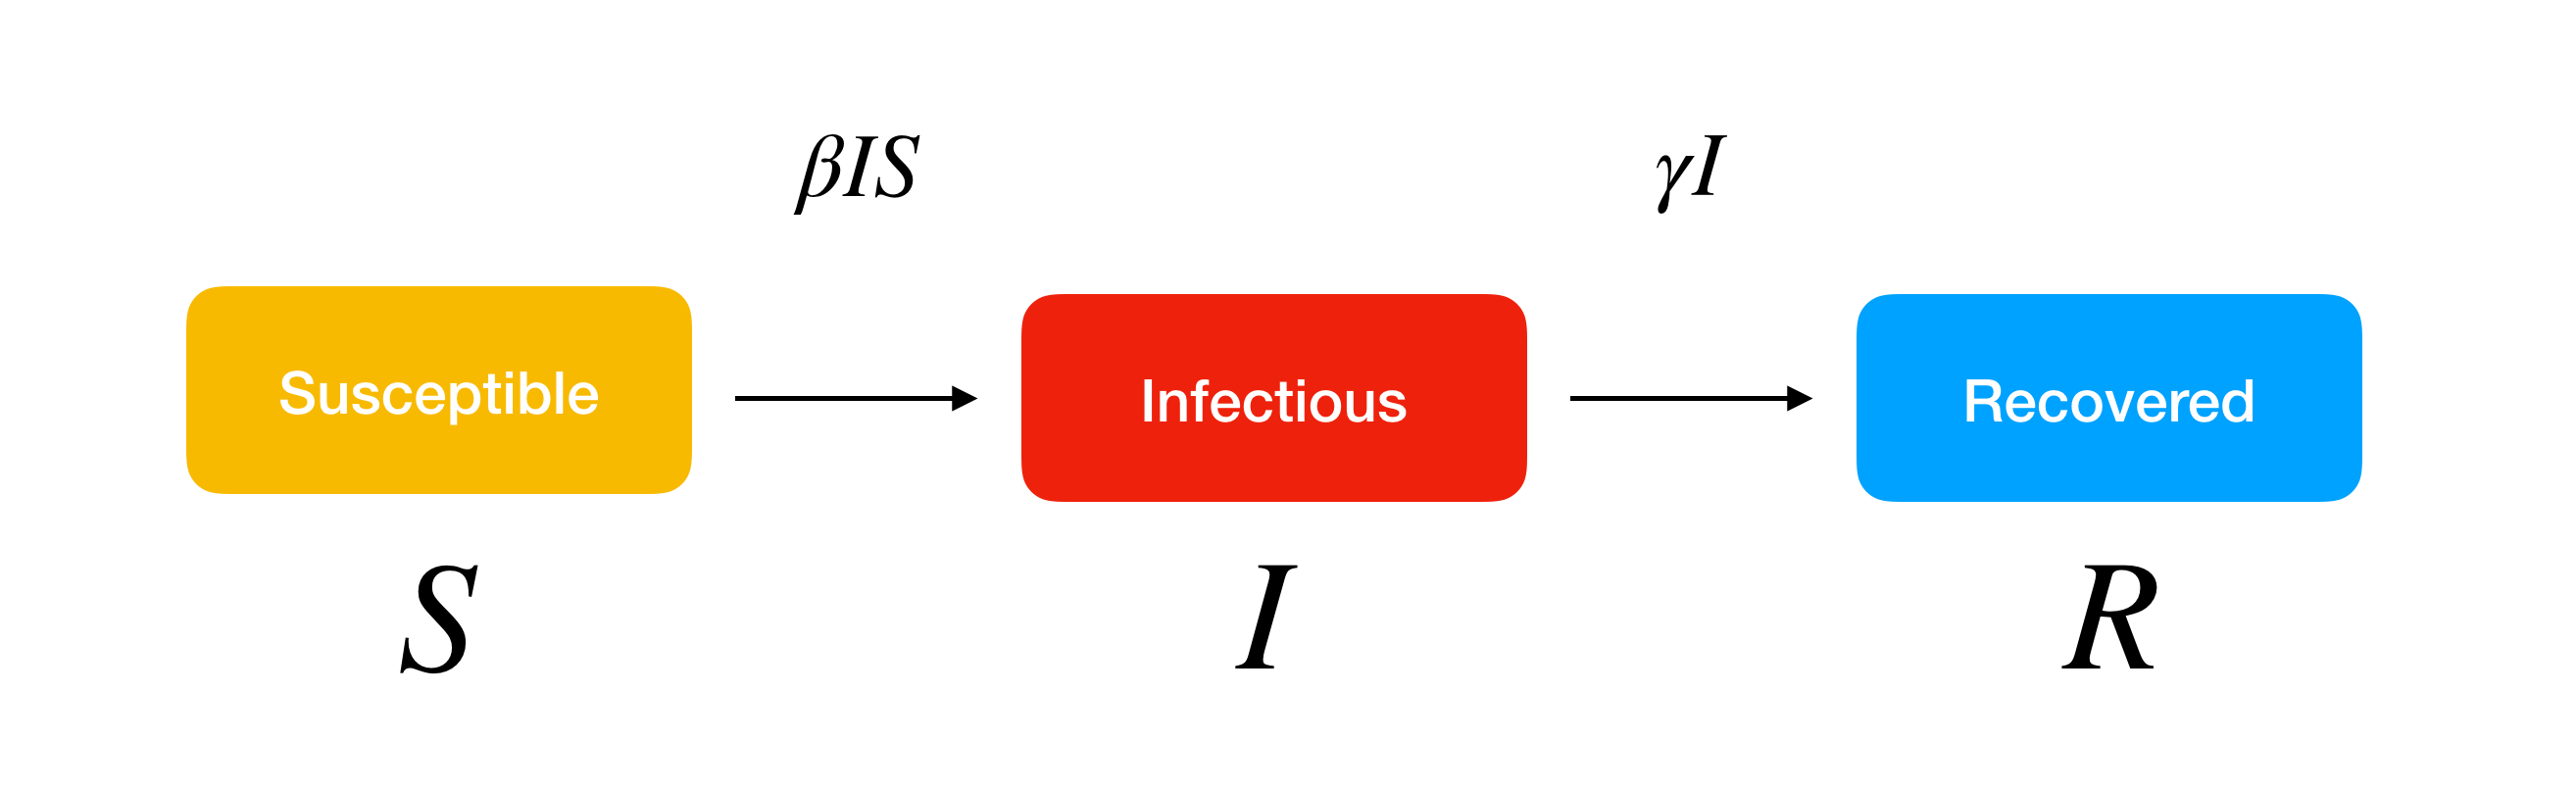
\includegraphics[width=\linewidth]{img/sir.png}
        \caption{Esempio della struttura del modello SIR} 
        \label{fig:SIR_Structure}
    \end{center}
\end{figure}

Da questa idea di base, è stato sviluppato un modello matematico che 
descrive come queste tre categorie, sebbene separate, interagiscano 
nel tempo. Il tempo è considerato la variabile indipendente del modello, 
denotata come $t$, e i tassi di transizione tra i compartimenti sono 
espressi come derivate rispetto al tempo e alle dimensioni dei 
compartimenti. Di conseguenza, questo modello è stato inizialmente 
formulato utilizzando equazioni differenziali ordinarie \cite{Brauer2008}.

Il sistema di equazioni differenziali che descrive il modello SIR è il seguente:

\[ \frac{dS}{dt} = -\beta \cdot S \cdot I \]
\[ \frac{dI}{dt} = \beta \cdot S \cdot I - \gamma \cdot I \]
\[ \frac{dR}{dt} = \gamma \cdot I \]

Questo sistema modella le seguenti assunzioni:

\begin{itemize}
    \item In media, un individuo nella popolazione ha abbastanza contatti 
    con gli altri da permettere la diffusione dell'infezione, con un tasso 
    di infezione rappresentato da $\beta \cdot N$, dove $N$ è il numero 
    totale di individui nella popolazione.
    \item Gli individui infetti lasciano il compartimento degli infetti a 
    un tasso di $\gamma \cdot I$.
    \item Non ci sono entrate o uscite di individui dalla popolazione 
    totale, tranne per le possibili uscite dovute alla morte causata 
    dalla malattia stessa.
\end{itemize}

L'indice $R_0$ rappresenta il numero di infezioni secondarie causate da 
un singolo individuo durante il suo periodo infettivo in una popolazione 
completamente suscettibile di dimensione $K \approx S(0)$. In questa 
situazione, un individuo infetto effettua $\beta \cdot K$ contatti per 
unità di tempo, ognuno dei quali può trasmettere l'infezione a un 
individuo suscettibile, producendo nuove infezioni durante il suo periodo 
medio di infettività di $\frac{1}{\gamma}$. Pertanto, il valore 
di $R_0$ è $\beta \cdot \frac{K}{\gamma}$.

Il valore di $R_0$ è cruciale nel determinare se si verificherà o meno 
un'epidemia. Se $R_0 < 1$, l'infezione si estinguerà prima di diventare 
un'epidemia. Se $R_0 > 1$, ci sarà un'epidemia.

La modellazione epidemiologica può diventare più complessa in presenza 
di una fase di esposizione, in cui gli individui infetti non sono 
immediatamente infettivi. In questo caso, è possibile aggiungere un 
compartimento "Exposed (E)" al modello, che influenzerà il sistema di 
equazioni differenziali. Questo tipo di modello è noto come SEIR 
(Susceptible, Exposed, Infectious, Recovered).

Il sistema di equazioni differenziali che descrive il modello SEIR è il seguente:

\[ \frac{dS}{dt} = - \beta(N) \cdot S \cdot I \]
\[ \frac{dE}{dt} = \beta(N) \cdot S \cdot I - \kappa \cdot E \]
\[ \frac{dI}{dt} = \kappa \cdot E - \gamma \cdot I \]
\[ \frac{dR}{dt} = \gamma \cdot I \]

\begin{figure}[H]
    \begin{center}
        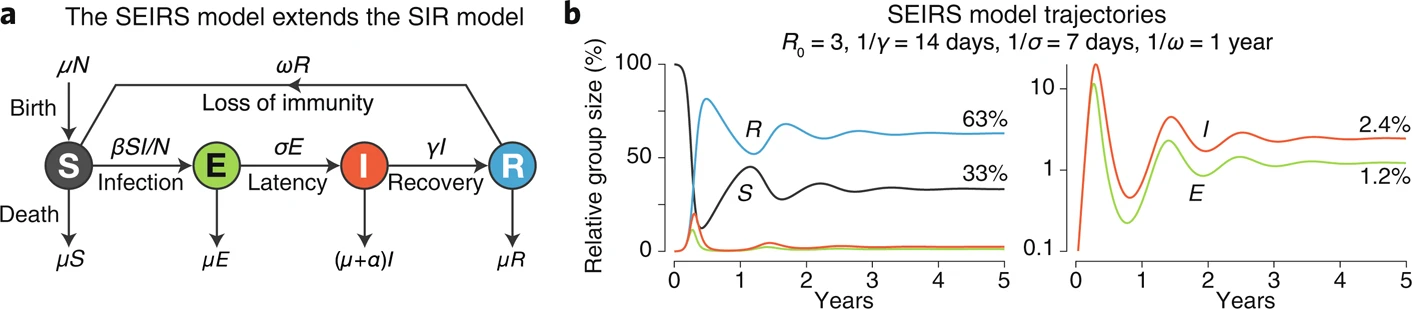
\includegraphics[width=\textwidth]{img/41592_2020_856_Fig1_HTML.png}
        \caption{Esempio di modello SEIRS \cite{Bjornstad2020}}
        \label{fig:SEIRS_model}
    \end{center}
\end{figure}

Un altro sviluppo importante è l'analisi dei modelli epidemiologici in 
forma stocastica, che tiene conto della variabilità individuale e delle 
piccole dimensioni dei compartimenti all'inizio di un'epidemia. 
Questi modelli stocastici considerano gli effetti casuali nei contatti 
tra gli individui e possono essere particolarmente rilevanti nelle prime 
fasi di un'epidemia, quando il numero di infetti è ancora relativamente 
basso. In queste situazioni, è necessario utilizzare approcci stocastici, 
come i modelli basati su reti (network models) per catturare la dinamica 
epidemica in modo più accurato.

In generale, i modelli compartimentali sono strumenti essenziali per la 
modellazione e la comprensione della diffusione delle malattie infettive, 
consentendo agli epidemiologi di studiare scenari diversi e sviluppare 
strategie di controllo più efficaci.

\begin{figure}[H]
    \begin{center}
        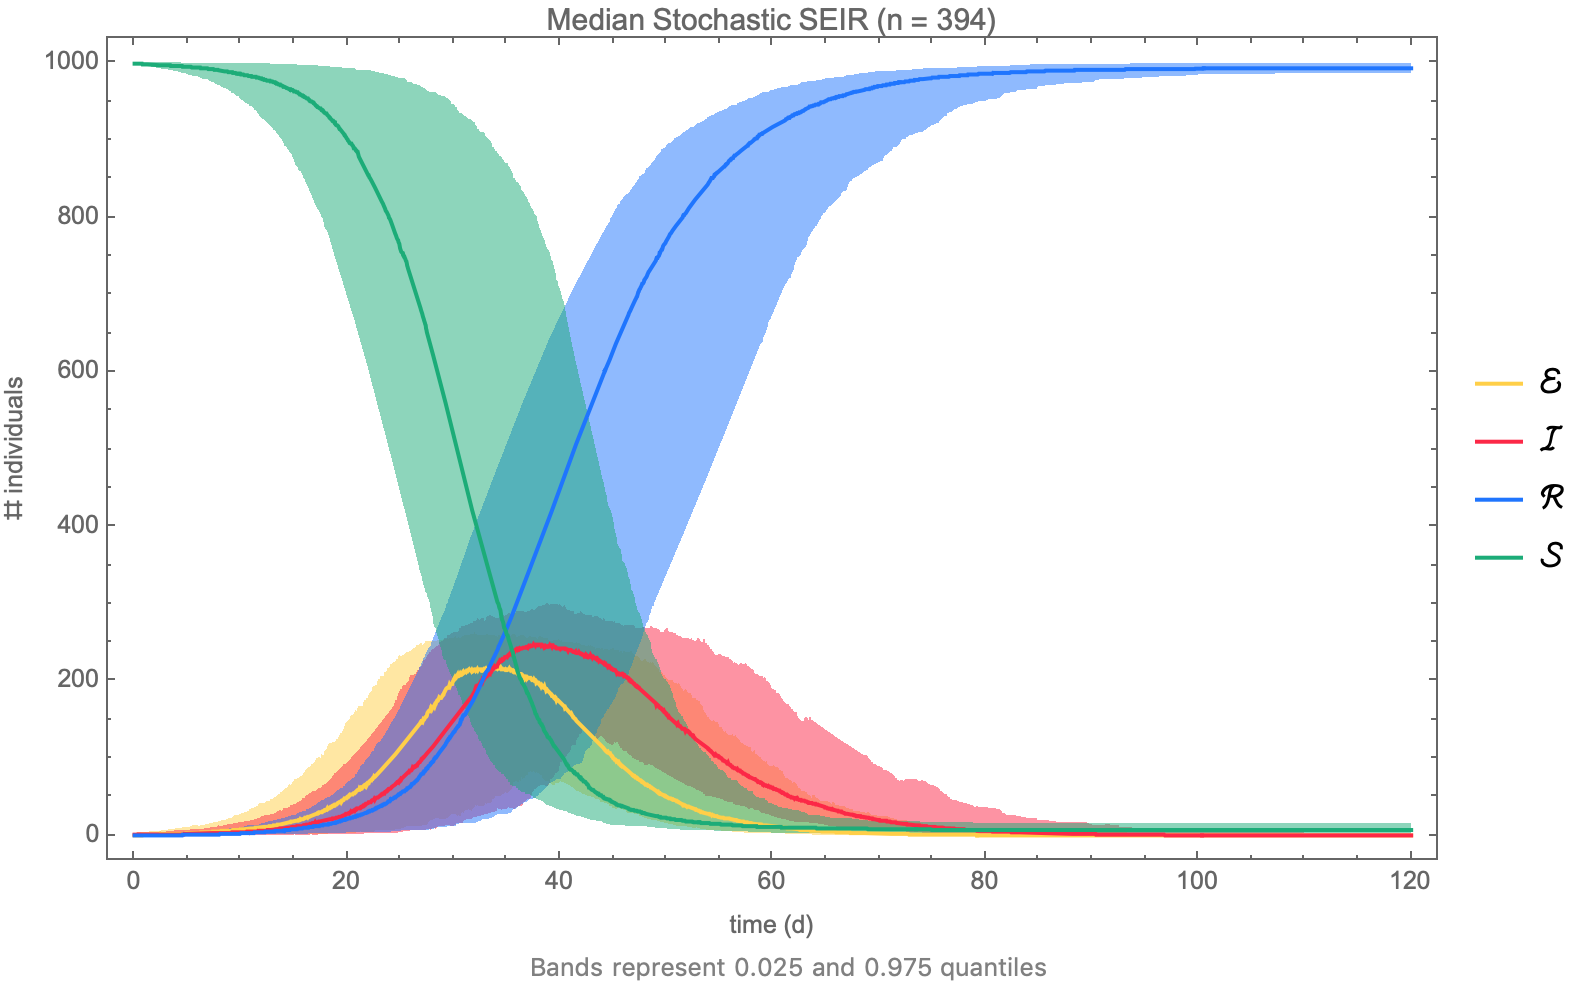
\includegraphics[width=\textwidth]{img/stochastic_SEIR.png}
        \caption{Esempio di modello SEIR stocastico}
        \url{https://community.wolfram.com//c/portal/getImageAttachment?filename=stochastic_SEIR.png&userId=228444}
        \label{fig:stochastic_SEIR_model}
    \end{center}
\end{figure}